\documentclass[twoside, 11pt]{exam}

\usepackage[T1]{fontenc}
\usepackage[utf8]{inputenc}
\usepackage[dutch]{babel}

\usepackage[font={small,sf},labelfont={bf},labelsep=endash]{caption}
\usepackage{fouriernc}
\usepackage[detect-all, binary-units, separate-uncertainty=true,
            per-mode=symbol, retain-explicit-plus, range-phrase={ tot },
            list-final-separator={ en }, output-decimal-marker={,}]
            {siunitx}

\usepackage{setspace}
\setstretch{1.2}

\setlength{\parskip}{\smallskipamount}
\setlength{\parindent}{0pt}

\usepackage{geometry}
\geometry{a4paper, vmargin=3cm, inner=3cm, outer=2cm, head=14pt}

\usepackage{float}

\usepackage[fleqn]{amsmath}
\numberwithin{equation}{section}
\numberwithin{figure}{section}

\usepackage{graphicx}
\graphicspath{{Figures/}}
\usepackage{subfig}

\usepackage[svgnames]{xcolor}
\usepackage{tikz}
\usepackage{tikz-3dplot}
\usepackage{pgfplots}
\usetikzlibrary{plotmarks,circuits.ee.IEC,pgfplots.groupplots,external,calc}
\pgfplotsset{compat=1.3}

\usepackage{minted}
\usepackage{amsthm}
\usepackage{relsize}
\usepackage{xspace}
\usepackage{url}
\usepackage{sansmath}
\usepackage{titling}


\theoremstyle{plain}
\newtheorem*{note}{Note}


\newcommand{\figref}[1]{Figuur~\ref{#1}}

\newcommand{\hisparc}{\textsmaller{HiSPARC}\xspace}
\newcommand{\kascade}{\textsmaller{KASCADE}\xspace}
\newcommand{\sapphire}{\textsmaller{SAPPHiRE}\xspace}
\newcommand{\jsparc}{\textsmaller{jSparc}\xspace}
\newcommand{\hdf}{\textsmaller{HDF5}\xspace}
\newcommand{\aires}{\textsmaller{AIRES}\xspace}
\newcommand{\csv}{\textsmaller{CSV}\xspace}
\newcommand{\python}{\textsmaller{PYTHON}\xspace}
\newcommand{\corsika}{\textsmaller{CORSIKA}\xspace}
\newcommand{\labview}{\textsmaller{LabVIEW}\xspace}
\newcommand{\dspmon}{\textsmaller{DSPMon}\xspace}
\newcommand{\daq}{\textsmaller{DAQ}\xspace}
\newcommand{\adc}{\textsmaller{ADC}\xspace}
\newcommand{\adcs}{\textsmaller{ADC}s\xspace}
\newcommand{\Adcs}{A\textsmaller{DC}s\xspace}
\newcommand{\hi}{\textsc{h i}\xspace}
\newcommand{\hii}{\textsc{h ii}\xspace}
\newcommand{\mip}{\textsmaller{MIP}\xspace}
\newcommand{\hisparcii}{\textsmaller{HiSPARC II}\xspace}
\newcommand{\hisparciii}{\textsmaller{HiSPARC III}\xspace}
\newcommand{\pmt}{\textsmaller{PMT}\xspace}
\newcommand{\pmts}{\textsmaller{PMT}s\xspace}
\newcommand{\gps}{\textsmaller{GPS}\xspace}

\DeclareSIUnit{\electronvolt}{\ensuremath{\mathrm{e\!\!\:V}}}

\DeclareSIUnit{\unitsigma}{\ensuremath{\sigma}}
\DeclareSIUnit{\mip}{\textsmaller{MIP}}
\DeclareSIUnit{\adc}{\textsmaller{ADC}}

\DeclareSIUnit{\gauss}{G}
\DeclareSIUnit{\parsec}{pc}
\DeclareSIUnit{\year}{yr}


%% Document style definitions

% macros and commands
\newcommand{\shorttitle}[1]{\def\theshorttitle{#1}}
\newcommand{\docindex}[1]{\def\thedocindex{#1}}
\newcommand{\version}[1]{\def\theversion{#1}}
\newcommand{\setsectionstyle}[2]{
  \colorlet{seccolor}{#1}
  \def\thesectiontitle{#2}
}

\newcommand{\setdocumentstyle}[4]{
  \setsectionstyle{#1}{#2}
  \docindex{#3}
  \shorttitle{#4}
}

% document types
\newcommand{\docalgemeen}[2]{\setdocumentstyle{red}{Algemeen}{#1}{#2}}
\newcommand{\docinstallatie}[2]{\setdocumentstyle{Gold}{Detector installatie}{#1}{#2}}
\newcommand{\docdetector}[2]{\setdocumentstyle{blue}{Detector}{#1}{#2}}
\newcommand{\docweerstation}[2]{\setdocumentstyle{LightSlateGray}{Weerstation}{#1}{#2}}
\newcommand{\docbliksem}[2]{\setdocumentstyle{orange}{Bliksem}{#1}{#2}}
\newcommand{\docanalyse}[2]{\setdocumentstyle{DarkViolet}{Data analyse}{#1}{#2}}
\newcommand{\docwerkblad}[2]{\setdocumentstyle{ForestGreen}{Werkbladen}{#1}{#2}}
\newcommand{\docdocent}[2]{\setdocumentstyle{DarkKhaki}{Uitwerkingen}{#1}{#2}}
\newcommand{\docopdrachten}[2]{\setdocumentstyle{Silver}{Opdrachten}{#1}{#2}}
\newcommand{\docrecept}[2]{\setdocumentstyle{Navy}{Recept}{#1}{#2}}

\pgfmathsetlengthmacro\stylemarginsep{+1cm}
\pgfmathsetlengthmacro\stylethumbsep{+.75cm}

\newcommand{\rightthumb}{
\begin{tikzpicture}[remember picture, overlay]
  % vertical line
  \draw[seccolor]
    ($(current page.north east) + (-\stylemarginsep, -.5cm)$) --
    ($(current page.south east) + (-\stylemarginsep, .5cm)$);

  % thumb
  \fill[seccolor]
    ($(current page.north east) +
      (-\stylemarginsep, -2cm -\thedocindex * \stylethumbsep)$)
      rectangle +(.5cm, -.5cm);
\end{tikzpicture}
}

\newcommand{\leftthumb}{
\begin{tikzpicture}[remember picture, overlay]
  % vertical line
  \draw[seccolor]
    ($(current page.north west) + (\stylemarginsep, -.5cm)$) --
    ($(current page.south west) + (\stylemarginsep, .5cm)$);

  % thumb
  \fill[seccolor]
    ($(current page.north west) +
      (\stylemarginsep, -2cm -\thedocindex * \stylethumbsep)$)
      rectangle +(-.5cm, -.5cm);
\end{tikzpicture}
}

\renewcommand{\maketitle}{
  \suppressfloats

  \begin{titlepage}
  \thispagestyle{\defaultstyle}
  \let\endtitlepage\relax
  \begin{tikzpicture}[remember picture, overlay,
    titlebox/.append style={seccolor, fill, text=white, minimum height=1cm,
      font=\sffamily\huge, draw=none},
    authorbox/.append style={minimum height=.5cm, font=\sffamily}]

    \node[titlebox, anchor=north west, shift={(3cm, -1cm)}] at
      (current page.north west) {\thesectiontitle};

    \node[anchor=north west, shift={(2.83cm, -2cm)}] at
      (current page.north west) {
\includegraphics[scale=.8]{../HiSPARC_header}};

    \node[titlebox, anchor=north east, shift={(-\stylemarginsep, -1cm)}] at
      (current page.north east) {\thetitle};

    \node[authorbox, anchor=north east, shift={(-\stylemarginsep, -2cm)}] at
      (current page.north east) {\theauthor};
  \end{tikzpicture}
  \end{titlepage}
}


\newcommand{\defaultstyle}{headandfoot}

% style definitions
\pagestyle{\defaultstyle}
\chead{\oddeven{\rightthumb}{\leftthumb}}
\cfoot{\theshorttitle\ -- \thepage}
\lfoot{\oddeven{}{\textcolor{gray}{\smaller Versie \theversion}}}
\rfoot{\oddeven{\textcolor{gray}{\smaller Versie \theversion}}{}}

\renewcommand{\thequestion}{\textbf{Opdracht \arabic{question}:}}
\renewcommand{\solutiontitle}{\noindent\textbf{Antwoord:}\enspace}
\newcommand{\makelines}[1]{\ifprintanswers\else\fillwithlines{#1\linefillheight}\fi}

\ifdefined\showanswers
  \printanswers
\else
  \noprintanswers
\fi


\title{Bliksem onderzoek}
\author{C.G. van Veen}
\docwerkblad{7}{BOW}
\version{1.1}

\begin{document}

\maketitle

\section{Inleiding}

Dit werkblad geeft handvatten om correlatie onderzoek te doen aan bliksem en
kosmische showers gemeten door \hisparc stations.
We hebben een aantal websites nodig voor ons onderzoek, namelijk:
\begin{enumerate}
    \item Database met datum/posities van bliksemontladingen van het KNMI\\
    \url{ http://www.knmi.nl/klimatologie/daggegevens/onweer/} \\
    Momenteel heeft de bliksem database van \hisparc data beschikbaar van 2003-2013.
    \item Zoeken in de database van \hisparc.\\
    \url{http://data.hisparc.nl}
\end{enumerate}

Op website 1 kun je dagen met bliksem vinden in de database van het KNMI.
We zullen daar naar geschikte dagen met bliksemontladingen zoeken.
In de database van \hisparc kunnen we data van kosmische showers opvragen en
kijken of we bliksemontladingen kunnen relateren aan kosmische showers.
We kunnen ons daarbij afvragen binnen welk tijdsbestek een kosmische shower gemeten
moet worden en of dat voor of na een bliksem moet zijn. Om dit soort vragen te
beantwoorden kan literatuur over bliksem en kosmische straling bestudeert worden.
Zoals:\\
1. Achtergrond informatie bliksem en kosmischestraling (natuur en techniek)\\
\url{http://bruno.home.xs4all.nl/2005/NWT%200705%20bliksem.pdf}\\
2. Artikel van CWI.\\
\url{http://homepages.cwi.nl/~ebert/NWTbliksem09.pdf}\\

\section{Start}

\begin{questions}
\question
In welk gebied en welk station wil je bliksemontladingen vinden? Probeer met
van de website \url{http://data.hisparc.nl} de gps locaties van deze stations te
achterhalen. Schrijf het nummer van de stations op en hun GPS locatie.
Op de website \url{http://www.openstreetmap.org} kun je de gps locaties van zowel
stations en bliksemontladingen invoeren in de search balk van deze website.
\makelines{2}
\begin{solution}
    Open opdracht: ter beoordeling aan de docent. Aanbeveling: Doe het invoeren van GPS locatie
    even een keer voor op de website van `openstreetmap'.
\end{solution}

\question
Zoek op de site van het KNMI naar dagen waarop bliksemontladingen zijn geweest.
Schrijf een aantal dagen op, waarbij er ontladingen zijn in de buurt van jouw gewenste
locaties. Denk eraan om ook bijhorende tijd op te schrijven. Zie \figref{fig:KNMI_data}
\makelines{4}
\begin{solution}
    Dagen in bijvoorbeeld begin augustus 2005 geven veel bliksemontladingen.
\end{solution}

\question
Ga nu naar website 2 en bekijk \figref{fig:overview_website} en \figref{fig:data_download}
hoe je naar het datadownload formulier moet komen.
Als je op de website van het download formulier bent, bekijk dan \figref{fig:download_form}.
Download nu de data als een tsv bestand, zodat je deze kunt inlezen. Neem een zo kort mogelijk tijdsinterval
voor datadownload van zowel de events van het \hisparc station als de bliksemdata.
Dit scheelt met de analyse. schrijf de data en tijden op waarvan je data hebt gedownload.
\makelines{4}
\begin{solution}
    Open opdracht: ter beoordeling aan de docent.
\end{solution}

\question
Je hebt nu data opgehaald en kunt nu gaan analyseren.
Wat vindt je nog een tijdsduur waarin je zou kunnen zeggen dat bliksemontlading
en kosmische shower bij elkaar horen? Leg dit uit. \\
\small{Voor extra uitleg over de meetwaarden (traces) van \hisparc stations zie het stuk `dataretrieval'
op \url{ http://www.hisparc.nl/docent-student/lesmateriaal/informatie-pakket/} paragraaf 3.5.
Je moet voor een schatting van de tijdsduur "traces" bekijken met de dataretrieval tool.}
\makelines{4}
\begin{solution}
    De tijdsduur van de bliksemontlading om nog bij een kosmische shower te horen
    is heel kort. In de orde $<$ 100 nanoseconden, helaas heeft het KNMI een tijdsresolutie
    van microseconden. We zullen dus nooit echt een bijpassende bliksem vinden.
    Het geeft de leerling wel een moment om eens over tijdsduren van kosmische showers en bliksem
    na te denken. En hoe moeilijk het is om onderzoek te doen.
\end{solution}

\question
Als je tsv bestanden hebt gedownload kun je deze inlezen in Excel. Hoe dat moet
wordt uitgelegd op deze website: \url{http://www.jkp-ads.com/Articles/importtextnl.asp}.
Je kunt nu data uitzetten in plotjes.
Plot bijvoorbeeld eens het aantal bliksem ontladingen tegen tijd.
Je kunt hiervoor de grafiek wizard van Excel gebruiken.
\makelines{4}
\begin{solution}
    De plotjes zijn ter beoordeling aan de docent.
\end{solution}

\begin{figure}
    \centering
    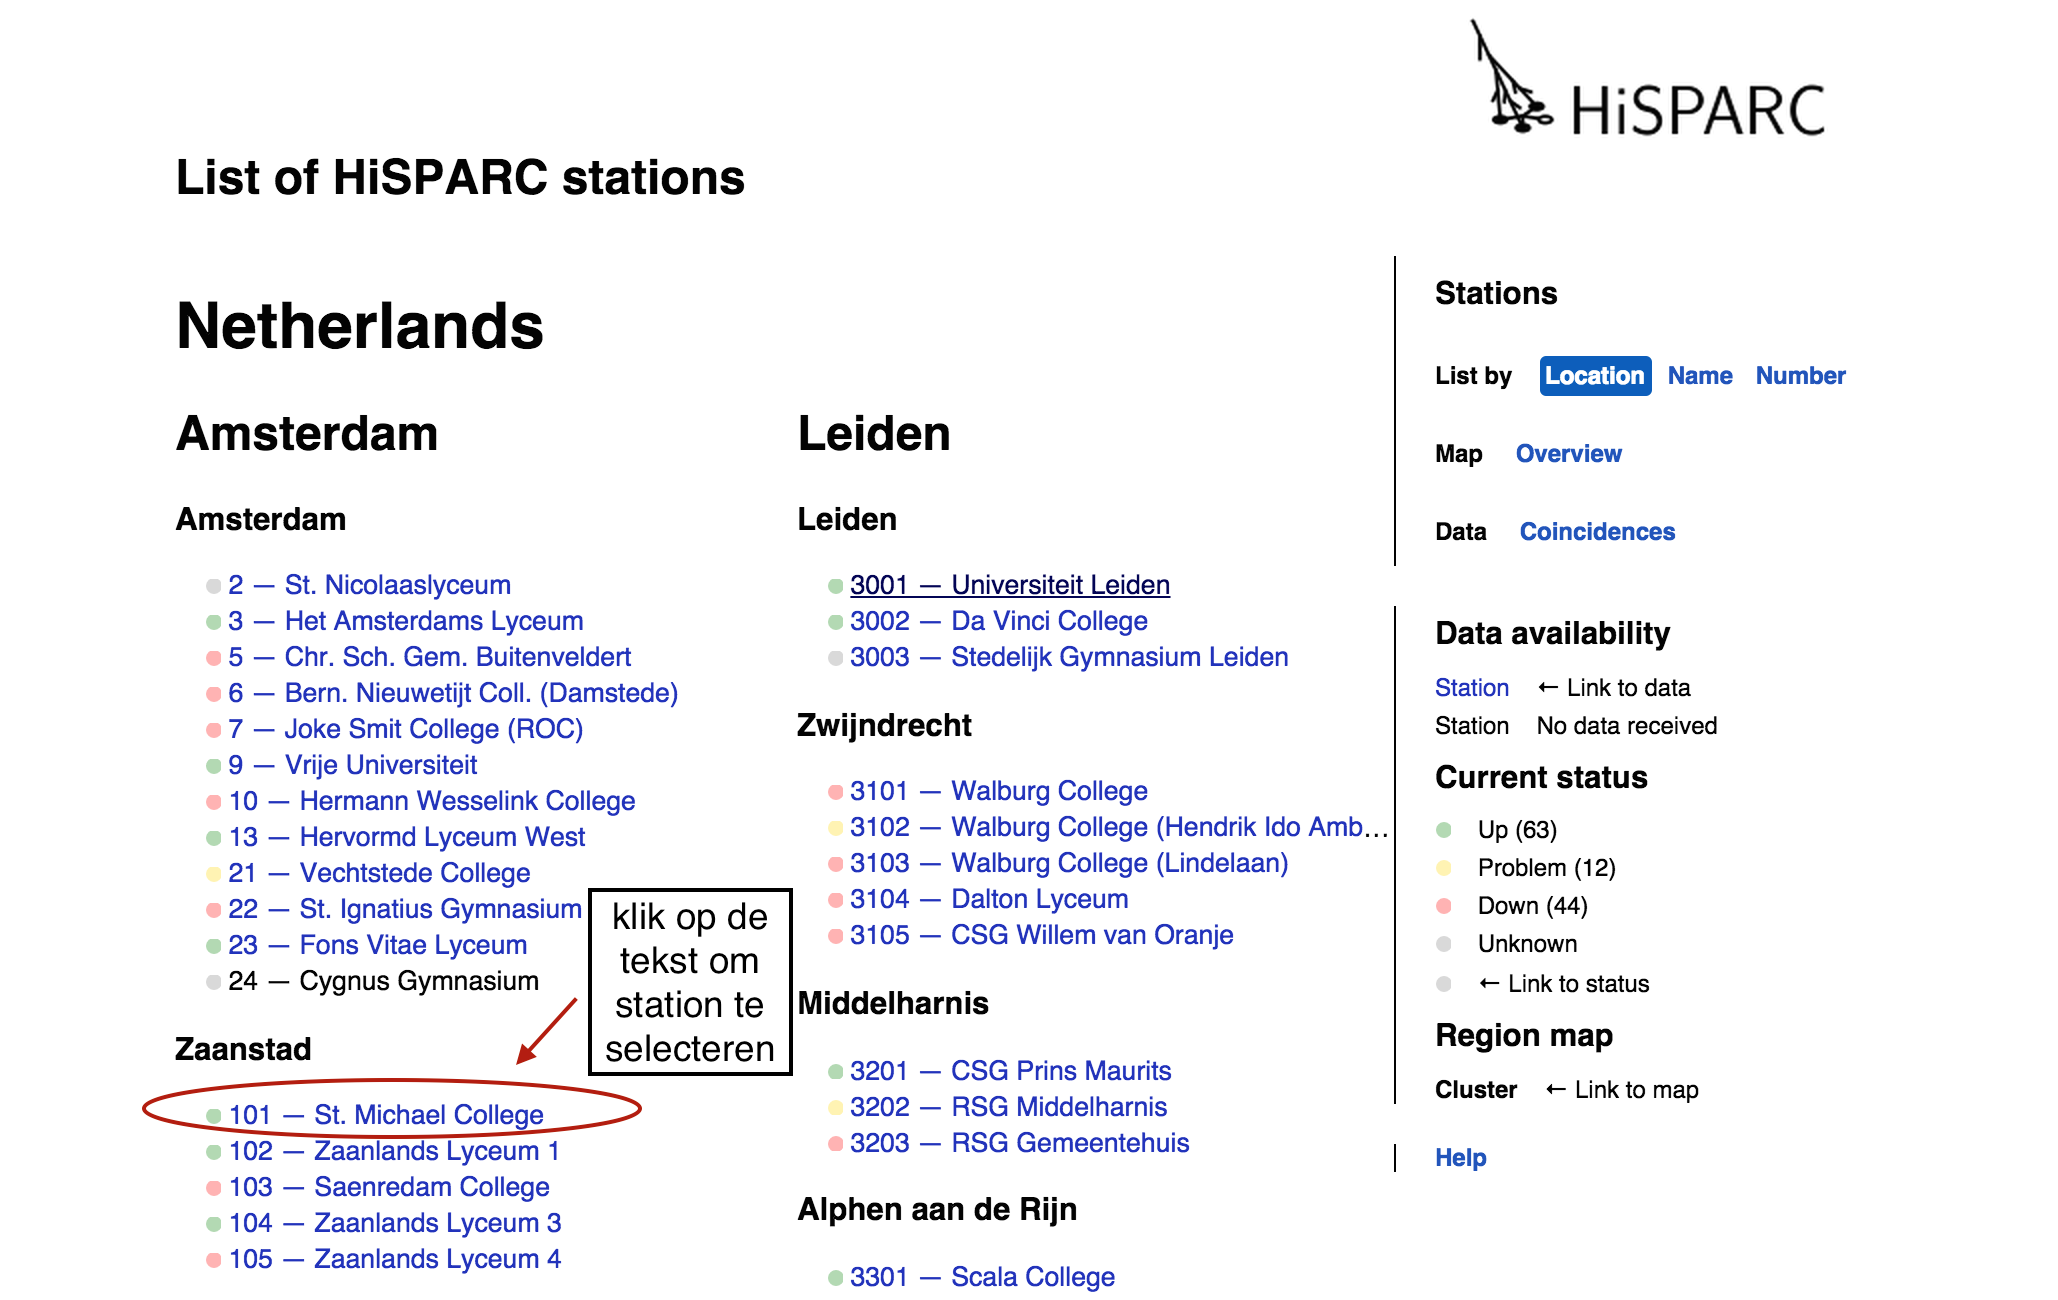
\includegraphics[scale=0.4]{overview_website}
    \caption{Weergegeven is de website \protect\url{http://data.hisparc.nl}.
    Klik nu op een station om op de pagina van
    het station te komen.}
    \label{fig:overview_website}
\end{figure}

\begin{figure}
    \centering
    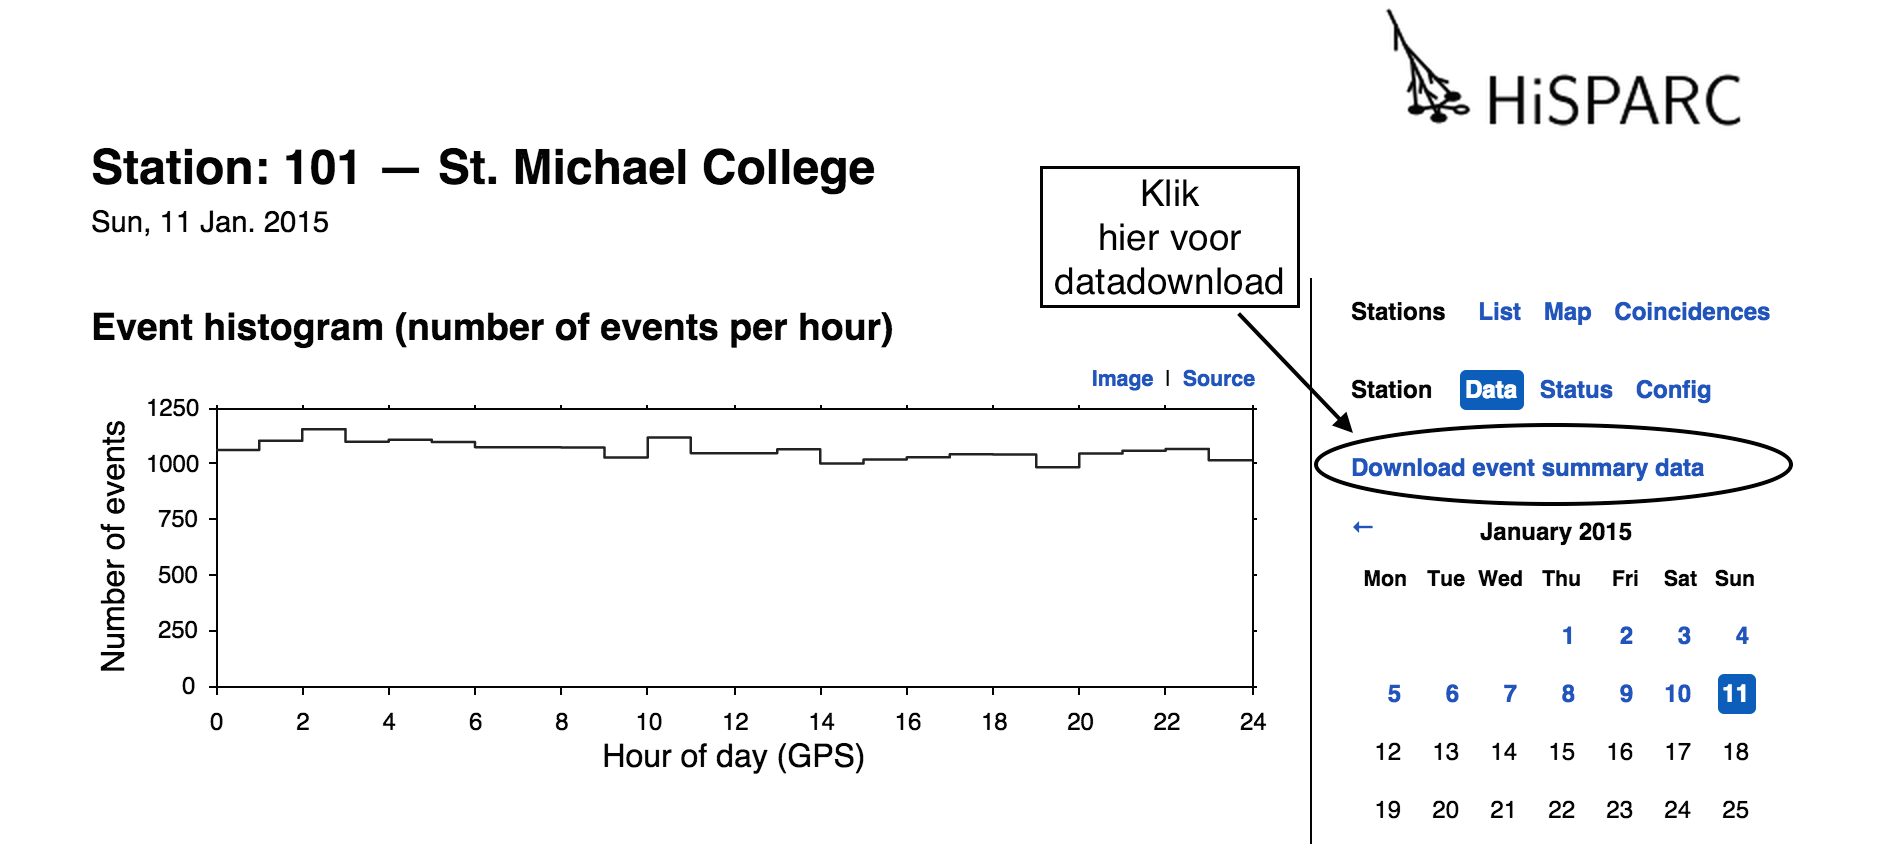
\includegraphics[scale=0.4]{data_download}
    \caption{Klik op "download event summary data", om bij het dataformulier te komen.}
    \label{fig:data_download}
\end{figure}

\begin{figure}
    \centering
    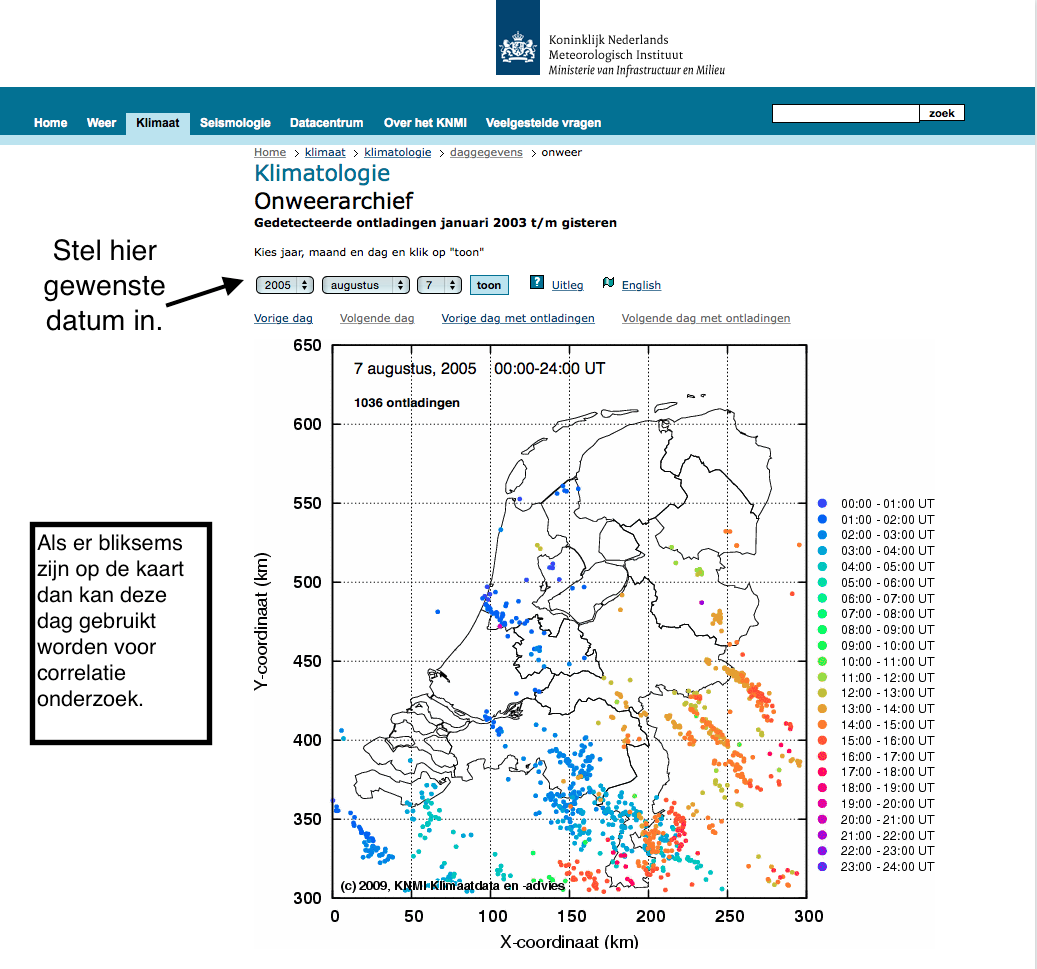
\includegraphics[scale=0.3]{KNMI_data}
    \caption{Op deze site van het KNMI (website 1) kun je snel dagen met bliksem vinden. Als een dag
    met bliksem is gevonden, moet gecheckt worden of het \hisparc station wat in de
    buurt staat van veel bliksemontladingen, online was die dag. Zo ja, dan kan
    er met het dataformulier zowel bliksemdata als kosmische straling events
    gedownload worden.}
    \label{fig:KNMI_data}
\end{figure}

\begin{figure}
    \centering
    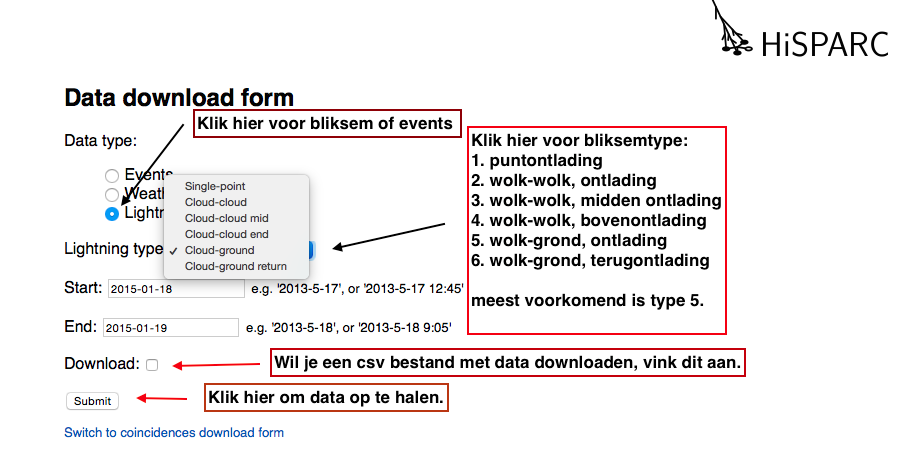
\includegraphics[scale=0.4]{download_form}
    \caption{Op de website van het downloadformulier kun je het formulier
    instellen voor downloaden van bliksem, stel de datum en tijd in als volgt:
    2013-5-17 12:45. Geef zowel begin: datum en tijd als eind: datum en tijd op. Meestal
    kiezen we voor bliksemtype: wolk-grond. Als je events wilt downloaden, dan
    moet je station nummer en datum en tijd ingeven }
    \label{fig:download_form}
\end{figure}

\uplevel{\section{Conclusie}}

\question
Wat is je conclusie na data analyse? Kun je een correlatie tussen bliksem en
kosmische showers vinden? Leg uit.
\makelines{4}
\begin{solution}
    Hopelijk hebben de leerlingen een conclusie in lijn met hun bevindingen.
\end{solution}

\end{questions}
\end{document}
